\chapter{Proposed Solution}
\label{cap:cap3}

The problem addressed by this thesis is running containerized services reliably across a cluster of machines. The key challenges are: discovering nodes automatically, distributing workloads efficiently, recovering from failures without downtime, and controlling access to the platform. Existing solutions like Kubernetes solve these problems but are too complex for smaller deployments and educational use.

The proposed solution is a distributed platform built from scratch in Go that implements the core mechanisms needed to manage a cluster: heartbeat-based node discovery, resource pools, pluggable load balancing, automatic fault recovery, JWT-based security with role-based access control, and an append-only audit log. The cluster state is replicated across multiple master nodes using the Raft consensus protocol.

This chapter describes the architecture in detail. The platform has two main components: the \textbf{master node}, which manages the cluster, and the \textbf{worker nodes}, which run the containers.

\section{Technology Choices}

The following technologies were chosen for the implementation:

\begin{itemize}
    \item \textbf{Go} -- chosen as the main language for its built-in concurrency model (goroutines and channels), efficient networking libraries, single-binary compilation, and strong support for systems programming. Both the master and worker are written in Go.
    \item \textbf{UDP multicast} -- used for heartbeats because it is lightweight (no connection setup, no handshake) and allows a single packet to reach all master nodes simultaneously. This is more efficient than TCP for periodic status messages that do not require acknowledgment.
    \item \textbf{Docker} -- used as the container runtime on worker nodes. The Docker SDK for Go provides a simple API for creating, starting, and stopping containers programmatically.
    \item \textbf{HashiCorp Raft} -- an open-source Go implementation of the Raft consensus protocol. Used for leader election and state replication between master nodes.
    \item \textbf{JWT (JSON Web Tokens)} -- used for user authentication. JWTs are stateless (no server-side session storage needed) and can encode the user's role directly in the token.
\end{itemize}

\section{Component Overview}

The platform follows a master-worker architecture. The master node handles all management tasks, while worker nodes execute containers and report their status.

\begin{figure}[H]
    \centering
    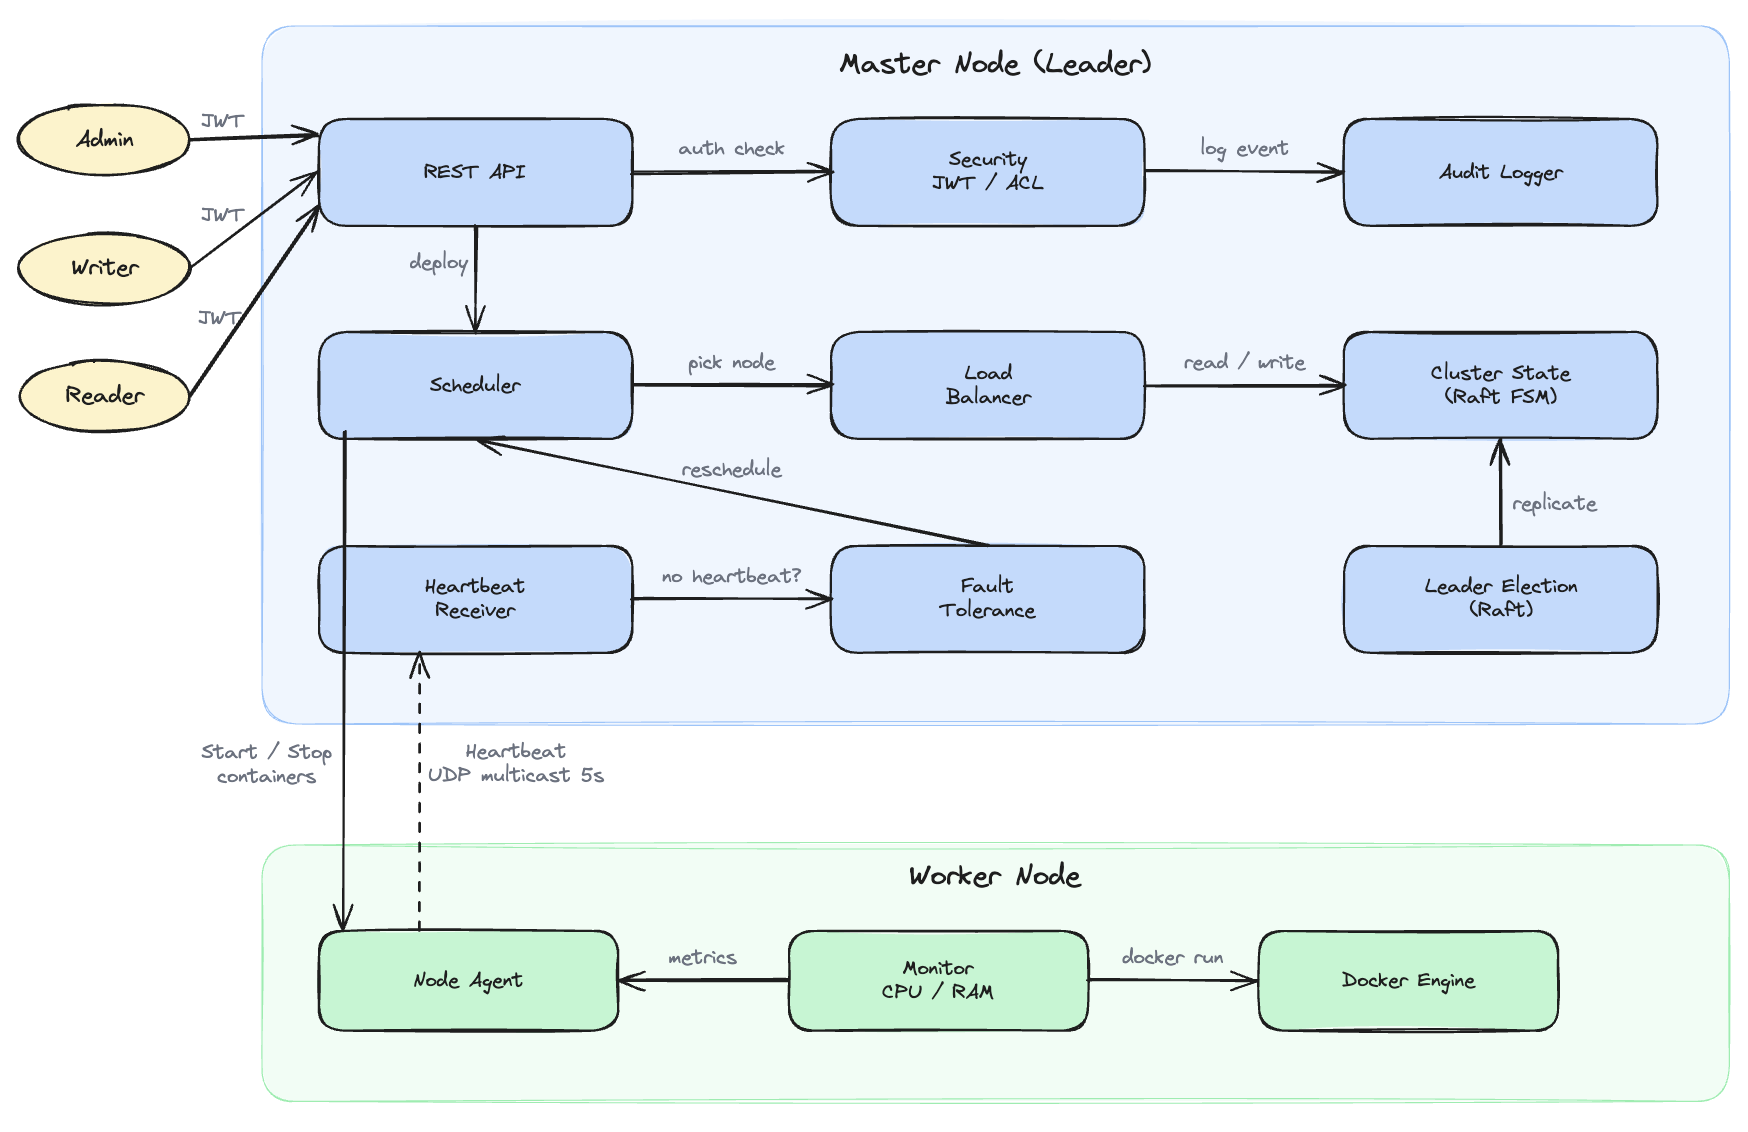
\includegraphics[width=\textwidth]{continut/capitol3/figuri/component_overview.png}
    \caption{Component Overview}
    \label{fig:component_overview}
\end{figure}

\subsection{Master Node}

The master node contains the following modules:

\textbf{Request pipeline:}
\begin{itemize}
    \item \textbf{REST API} -- the entry point for users. Exposes endpoints for managing services, nodes, and pools.
    \item \textbf{Security} -- handles JWT authentication and ACL authorization. Every request passes through this module before being processed.
    \item \textbf{Audit Logger} -- records all important events in an append-only log.
\end{itemize}

\textbf{Scheduling pipeline:}
\begin{itemize}
    \item \textbf{Scheduler} -- receives deploy requests and filters nodes in the requested pool that have enough resources. Passes the candidate list to the Load Balancer.
    \item \textbf{Load Balancer} -- selects the best node from the candidate list. Supports two strategies: Least Connections and Weighted.
    \item \textbf{Cluster State (Raft FSM)} -- the source of truth for the entire cluster. Stores all data about nodes, services, containers, pools, and users. Replicated across 3 master nodes via Raft.
\end{itemize}

\textbf{Cluster health:}
\begin{itemize}
    \item \textbf{Heartbeat Receiver} -- listens for UDP multicast packets from workers every 5 seconds.
    \item \textbf{Fault Tolerance} -- monitors heartbeats and detects node failures. Marks nodes as SUSPECT after 15 seconds and DEAD after 30 seconds without a heartbeat.
    \item \textbf{Leader Election (Raft)} -- manages leader election across 3 master nodes using the Raft consensus protocol.
\end{itemize}

\subsection{Worker Node}

Each worker node runs three components:

\begin{itemize}
    \item \textbf{Monitor} -- reads system metrics (CPU usage, RAM usage) from the operating system.
    \item \textbf{Node Agent} -- the main process. Sends heartbeats every 5 seconds and listens for commands from the master (StartContainer, KillContainers).
    \item \textbf{Docker Engine} -- the agent interacts with Docker to start and stop containers.
\end{itemize}

\subsection{Communication}

Master and worker nodes communicate through two channels:
\begin{itemize}
    \item \textbf{Heartbeat} -- UDP multicast, every 5 seconds. The worker sends its metrics and the master updates its state. Fire-and-forget, no acknowledgment needed.
    \item \textbf{Commands} -- TCP, from master to worker. Used for StartContainer and KillContainers. Only triggered on deploy, scale, or fault recovery.
\end{itemize}

All nodes run within a trusted internal network, so no TLS encryption is used for node-to-master communication. Raft communication between master nodes is encrypted with mTLS.

\section{Domain Model}

\begin{figure}[H]
    \centering
    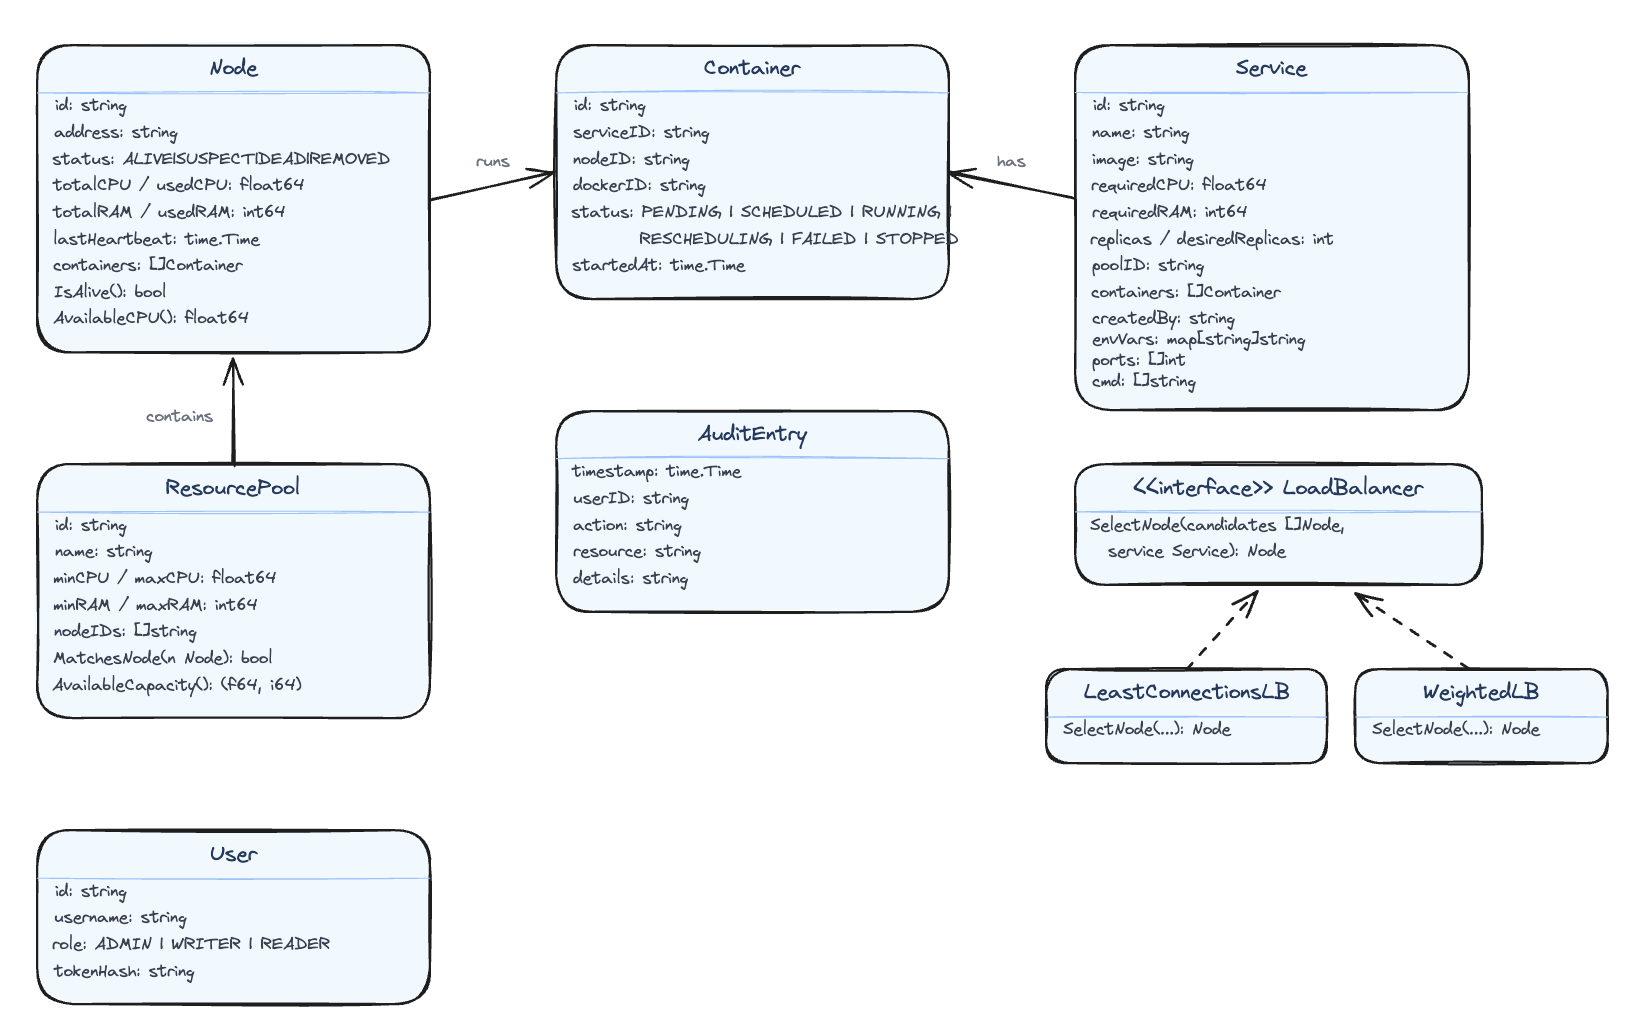
\includegraphics[width=\textwidth]{continut/capitol3/figuri/domain_model.png}
    \caption{Domain Model}
    \label{fig:domain_model}
\end{figure}

The platform uses the following data entities:

\textbf{Node} represents a worker machine in the cluster. It stores the node's address, total and used CPU/RAM, its current status (ALIVE, SUSPECT, DEAD, or REMOVED), and the timestamp of the last received heartbeat.

\textbf{Service} represents what the user wants to run. It contains the Docker image name, required CPU and RAM, the number of desired replicas, the target pool, and runtime parameters (environment variables, ports, command). These parameters are saved in the cluster state so that containers can be restarted identically during fault recovery.

\textbf{Container} is a running instance of a service on a specific node. It tracks the Docker container ID and its status (PENDING, SCHEDULED, RUNNING, FAILED, RESCHEDULING, or STOPPED).

\textbf{ResourcePool} groups nodes with similar hardware. Each pool has CPU and RAM ranges. When a new node is discovered, it is automatically assigned to the matching pool based on its resources.

\textbf{User} has an ID, username, role (ADMIN, WRITER, or READER), and a token hash for authentication.

\textbf{AuditEntry} records a single event with a timestamp, user ID, action, resource, and details.

\textbf{LoadBalancer} is an interface with a single method: SelectNode. It has two implementations: LeastConnectionsLB (picks the node with fewest active connections) and WeightedLB (picks the node with most available resources).

\section{Heartbeat and Node Discovery}

\begin{figure}[H]
    \centering
    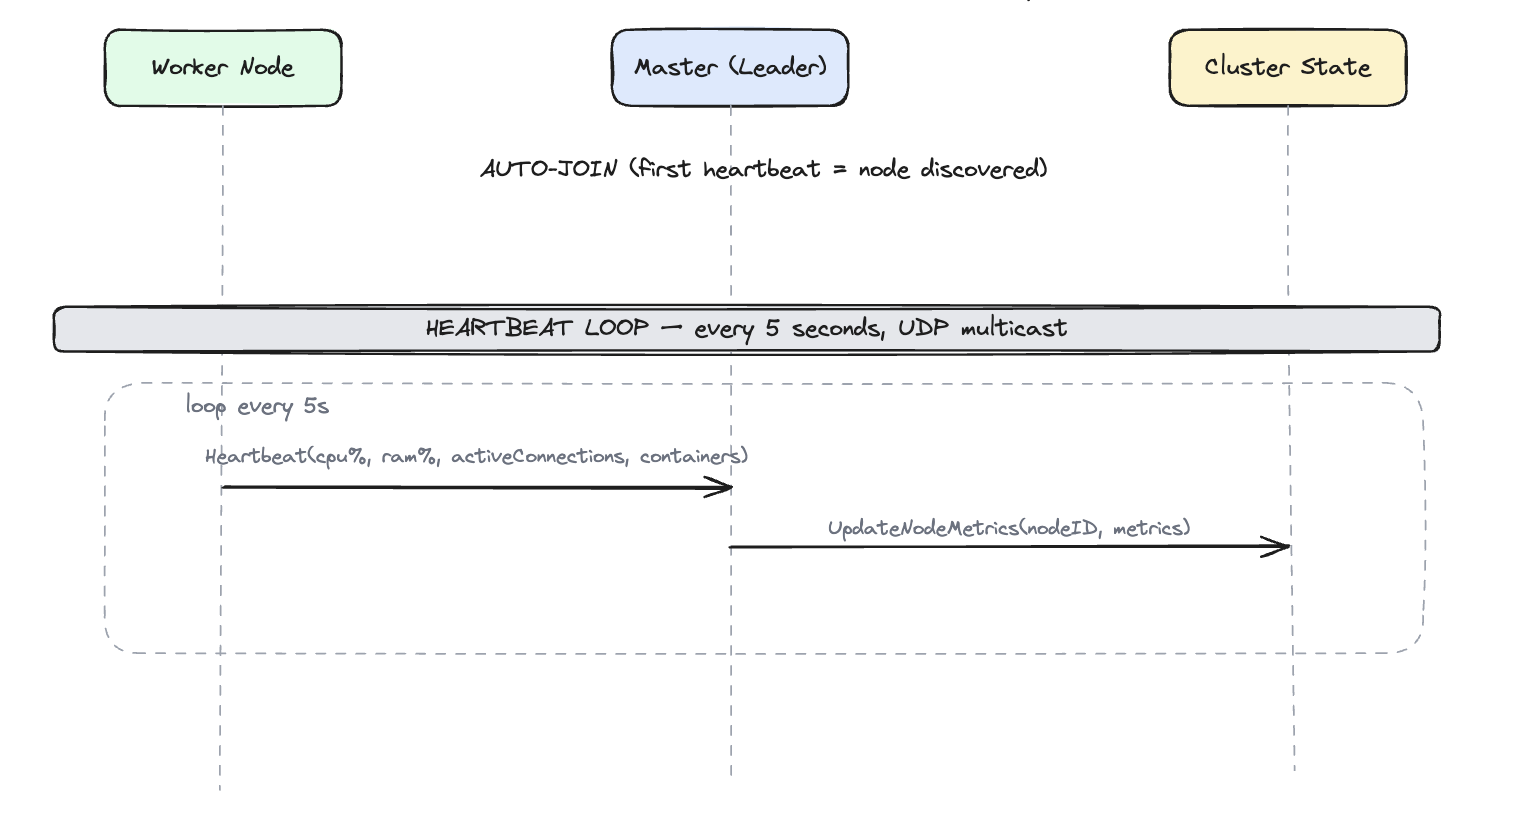
\includegraphics[width=\textwidth]{continut/capitol3/figuri/heartbeat.png}
    \caption{Heartbeat and Node Discovery}
    \label{fig:heartbeat}
\end{figure}

Node discovery is fully automatic. There is no explicit join or leave request.

\subsection{Auto-Join}

When the master receives the first heartbeat from an unknown node, it automatically:
\begin{enumerate}
    \item Adds the node to the cluster state with status ALIVE.
    \item Assigns it to the matching resource pool based on CPU and RAM reported in the heartbeat.
\end{enumerate}

\subsection{Heartbeat Loop}

Every 5 seconds, each worker sends a UDP multicast packet containing:
\begin{itemize}
    \item CPU usage (percentage)
    \item RAM usage (percentage)
    \item Number of active connections
    \item List of running containers
\end{itemize}

The master receives the packet and updates the node's metrics in the cluster state. No response is sent back -- the heartbeat is fire-and-forget.

\subsection{Node Removal}

There is no explicit leave request. When a worker stops (crash, shutdown, or network failure), it simply stops sending heartbeats. The master detects the absence through the fault tolerance mechanism (15 seconds SUSPECT, 30 seconds DEAD) and removes the node from the cluster.

\section{Fault Tolerance -- Detection and Recovery}

\begin{figure}[H]
    \centering
    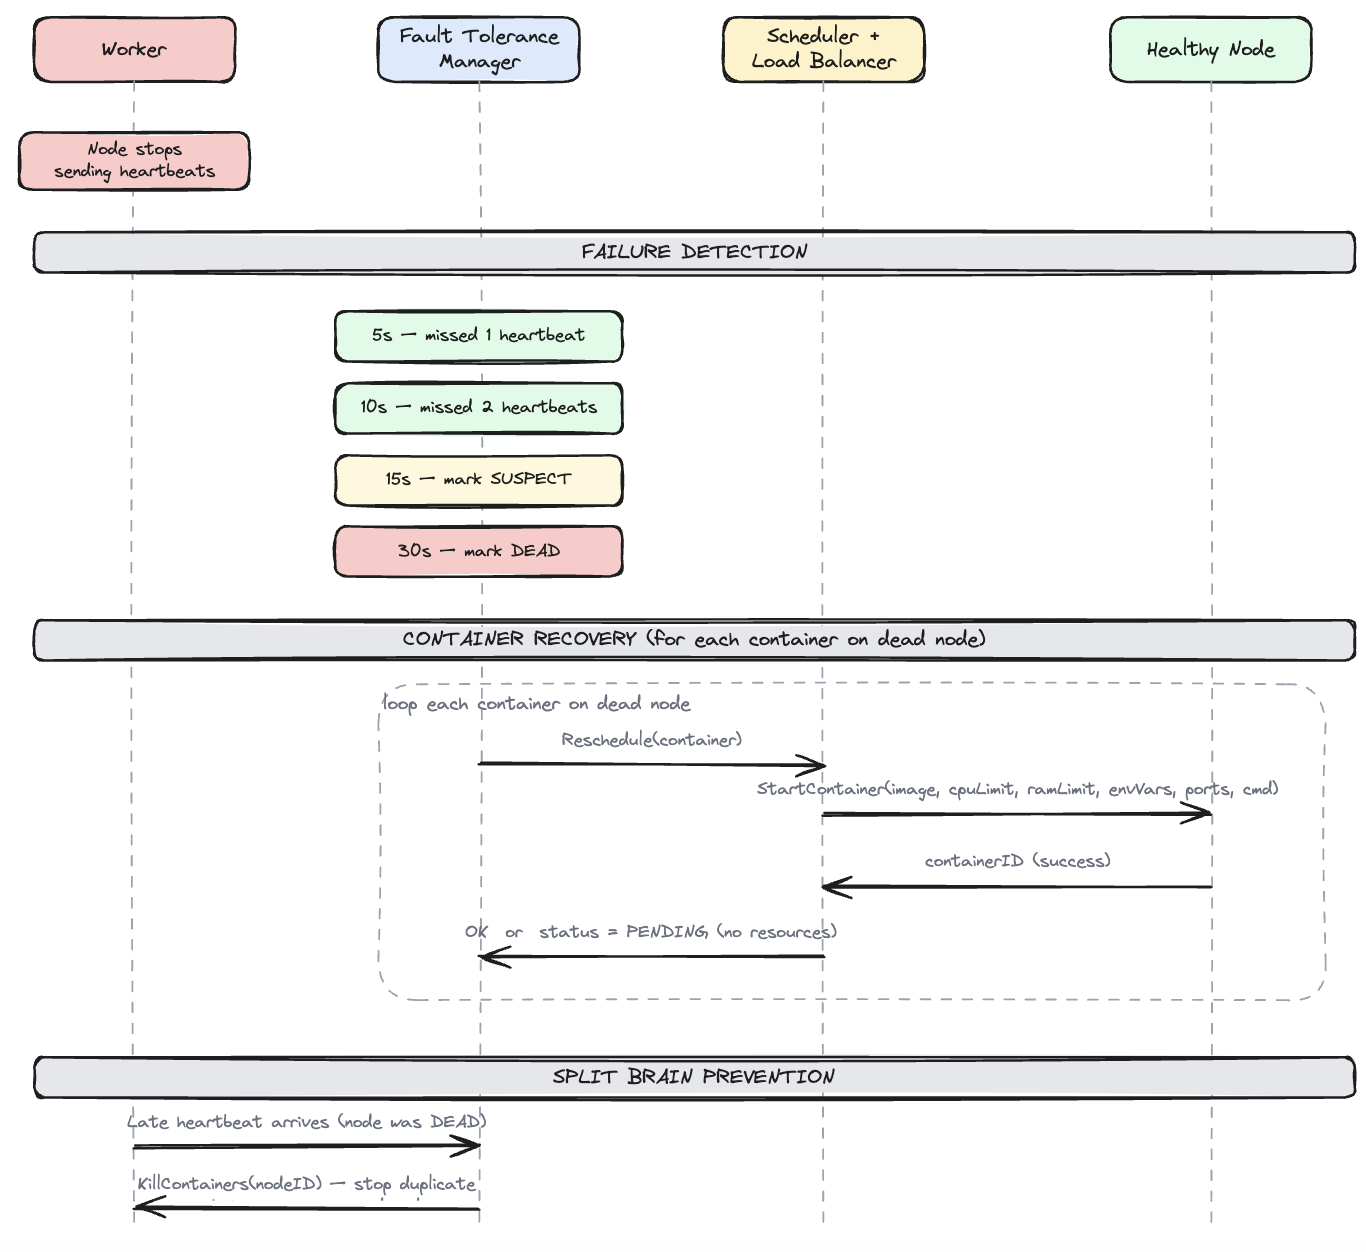
\includegraphics[width=\textwidth]{continut/capitol3/figuri/fault_tolerance.png}
    \caption{Fault Tolerance -- Detection and Recovery}
    \label{fig:fault_tolerance}
\end{figure}

\subsection{Failure Detection}

The Fault Tolerance module runs a periodic check (every 5 seconds) on all nodes. For each node, it computes the time since the last heartbeat:

\begin{itemize}
    \item \textbf{5 seconds} -- 1 missed heartbeat. Could be network jitter. No action.
    \item \textbf{10 seconds} -- 2 missed heartbeats. No action yet.
    \item \textbf{15 seconds} -- 3 missed heartbeats. The node is marked \textbf{SUSPECT}.
    \item \textbf{30 seconds} -- 6 missed heartbeats. The node is marked \textbf{DEAD}. Recovery begins.
\end{itemize}

\subsection{Container Recovery}

When a node is marked DEAD, its services still need to run. The system starts fresh containers on healthy nodes. For each service that had containers on the dead node:

\begin{enumerate}
    \item The Fault Tolerance module asks the Scheduler to find a new node.
    \item The Scheduler filters nodes in the matching pool with enough resources.
    \item The Load Balancer picks the best node.
    \item A StartContainer command is sent to the chosen node with the full service parameters (image, CPU limit, RAM limit, environment variables, ports, command).
    \item If no node has enough resources, the container stays in PENDING status until resources become available.
\end{enumerate}

The key point is that containers are not moved from the dead node -- they are started fresh from the service parameters saved in the cluster state.

\subsection{Split-Brain Prevention}

When a node that was marked DEAD comes back online (for example, after a temporary network failure), it sends a heartbeat. The master detects this as a late heartbeat and sends a \texttt{KillContainers} command to the recovered node. This stops all containers on the recovered node, because those containers have already been rescheduled onto other healthy nodes. Without this mechanism, the same containers would run on both the recovered node and the new nodes, creating duplicates.

After killing the duplicate containers, the recovered node continues sending heartbeats and becomes available for new scheduling.

\section{Worker Node -- State Machine}

\begin{figure}[H]
    \centering
    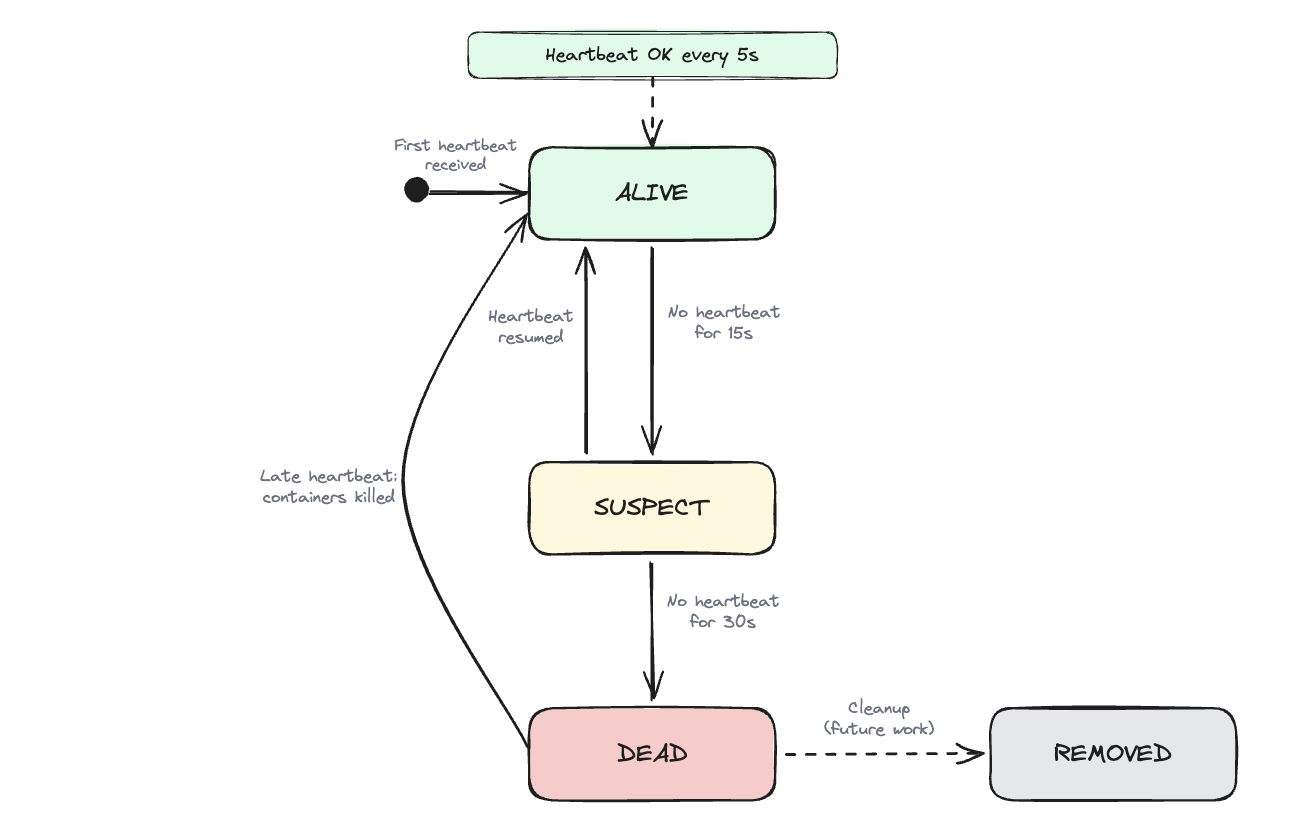
\includegraphics[width=\textwidth]{continut/capitol3/figuri/worker_state_machine.png}
    \caption{Worker Node -- State Machine}
    \label{fig:worker_state_machine}
\end{figure}

A worker node can be in one of four states:

\begin{itemize}
    \item \textbf{ALIVE} -- the initial and normal state. A node enters this state when the master receives its first heartbeat. It sends heartbeats every 5 seconds, runs containers, and is available for scheduling.
    \item \textbf{SUSPECT} -- the master has not received a heartbeat for 15 seconds. The node might be temporarily unreachable. No action is taken yet.
    \item \textbf{DEAD} -- no heartbeat for 30 seconds. The master starts fresh containers on other nodes using the original service parameters.
    \item \textbf{REMOVED} -- the node has been removed from the cluster state. All its containers have been rescheduled.
\end{itemize}

The transitions between states are:
\begin{itemize}
    \item First heartbeat received $\rightarrow$ ALIVE (auto-join)
    \item Heartbeat OK every 5s $\rightarrow$ stays ALIVE (self-loop)
    \item No heartbeat for 15s $\rightarrow$ SUSPECT
    \item Heartbeat resumed $\rightarrow$ back to ALIVE
    \item No heartbeat for 30s $\rightarrow$ DEAD
    \item Containers rescheduled $\rightarrow$ REMOVED
\end{itemize}

\section{Load Balancer}

The Load Balancer selects the best node from a list of candidates. It is defined as a Go interface with a single method:

\begin{verbatim}
type LoadBalancer interface {
    SelectNode(candidates []*Node, service *Service) *Node
}
\end{verbatim}

This design allows the load balancing strategy to be swapped without modifying the rest of the code. The platform provides two implementations:

\textbf{LeastConnectionsLB} picks the node with the fewest running containers. It iterates through the candidate list and selects the node with the smallest container count. This strategy works well when all containers have similar resource requirements.

\textbf{WeightedLB} picks the node with the most available resources. It calculates a score for each node based on available CPU and available RAM (converted to CPU-equivalent units), and selects the node with the highest score. This strategy is better when containers have varying resource needs.

The master can be started with either strategy using the \texttt{-lb} flag: \texttt{-lb leastconn} (default) or \texttt{-lb weighted}.

\section{Service Deployment Flow}

\begin{figure}[H]
    \centering
    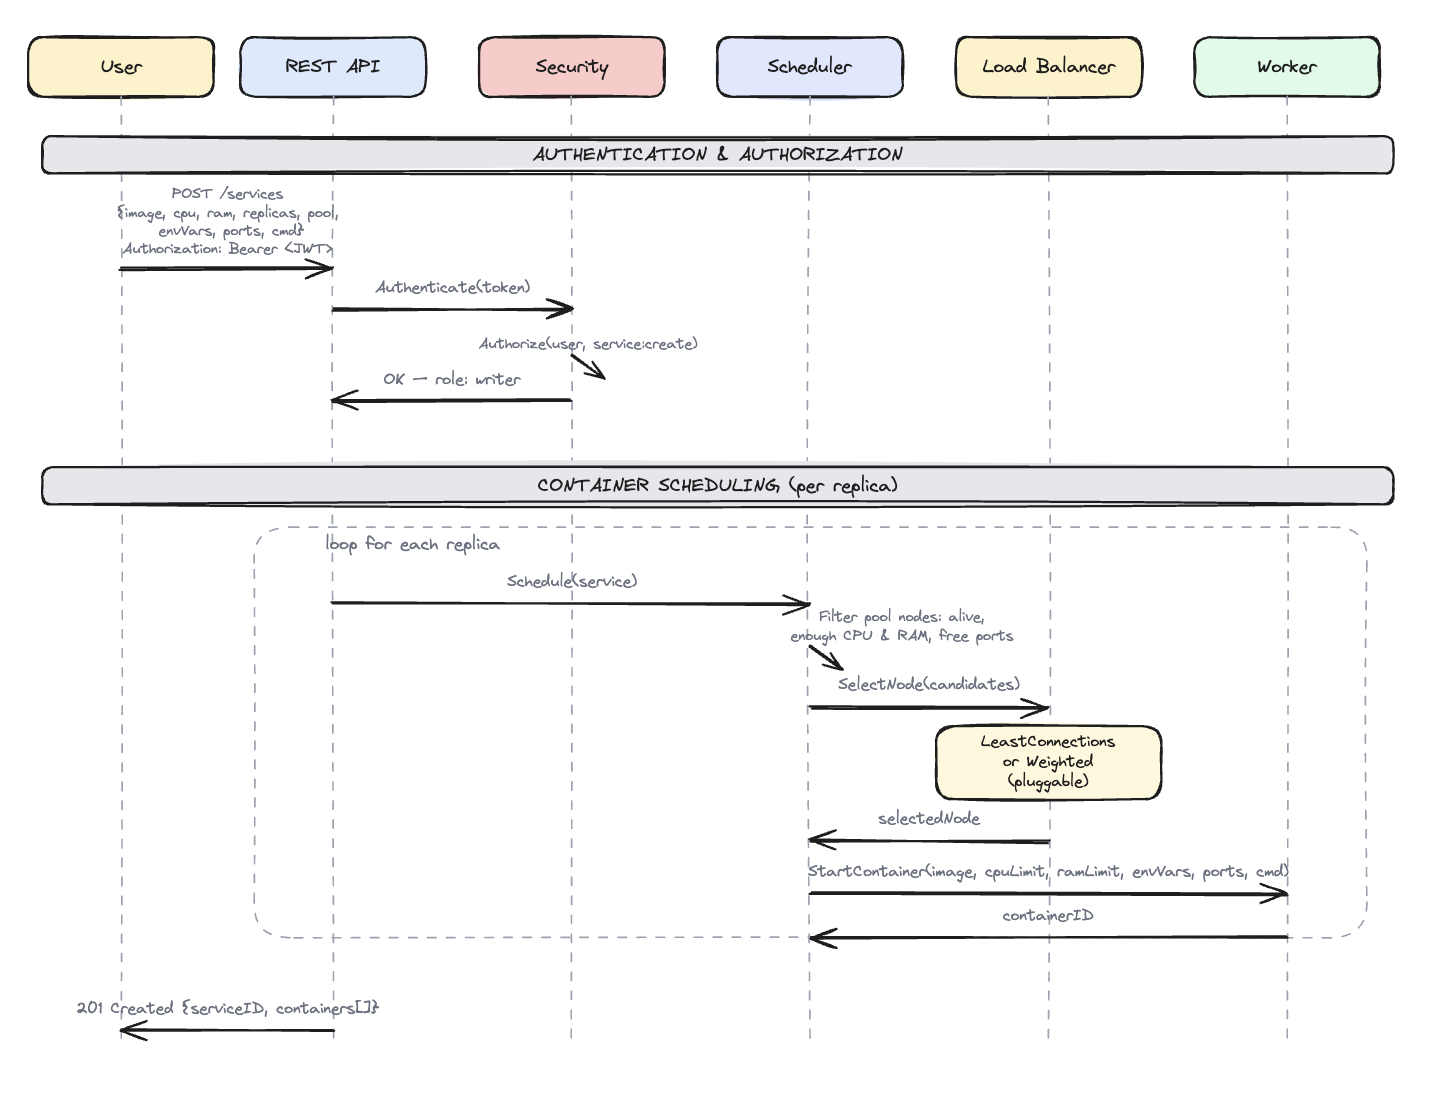
\includegraphics[width=\textwidth]{continut/capitol3/figuri/deployment_flow.png}
    \caption{Service Deployment Flow}
    \label{fig:deployment_flow}
\end{figure}

When a service needs to be deployed, the Scheduler and Load Balancer work together to find the best node. The Scheduler performs the following steps:

\begin{enumerate}
    \item Retrieves all nodes in the requested resource pool.
    \item Filters out nodes that are not ALIVE or do not have enough CPU and RAM for the service.
    \item Passes the candidate list to the Load Balancer.
    \item The Load Balancer returns the best node.
    \item A \texttt{StartContainer} command is sent to the selected node via TCP with the full service parameters (image, CPU limit, RAM limit, environment variables, ports, command).
    \item The worker receives the command, starts the container, and returns the container ID.
\end{enumerate}

This same flow is used both for new deployments and for fault recovery (when containers need to be rescheduled after a node dies).

\section{Agent -- Worker Command Server}

Each worker runs a TCP command server that listens for commands from the master. The server accepts two types of commands:

\textbf{StartContainer} -- the master sends the Docker image, resource limits, and service parameters. The worker starts a new container and returns the container ID.

\textbf{KillContainers} -- the master sends this command during split-brain prevention. The worker stops all running containers.

Commands are sent as JSON over TCP. The master uses the node's address (reported in heartbeats) to establish a connection, sends the command, and waits for a response. This communication is synchronous -- the master waits for the worker to confirm before proceeding.

\section{Container -- State Machine}

\begin{figure}[H]
    \centering
    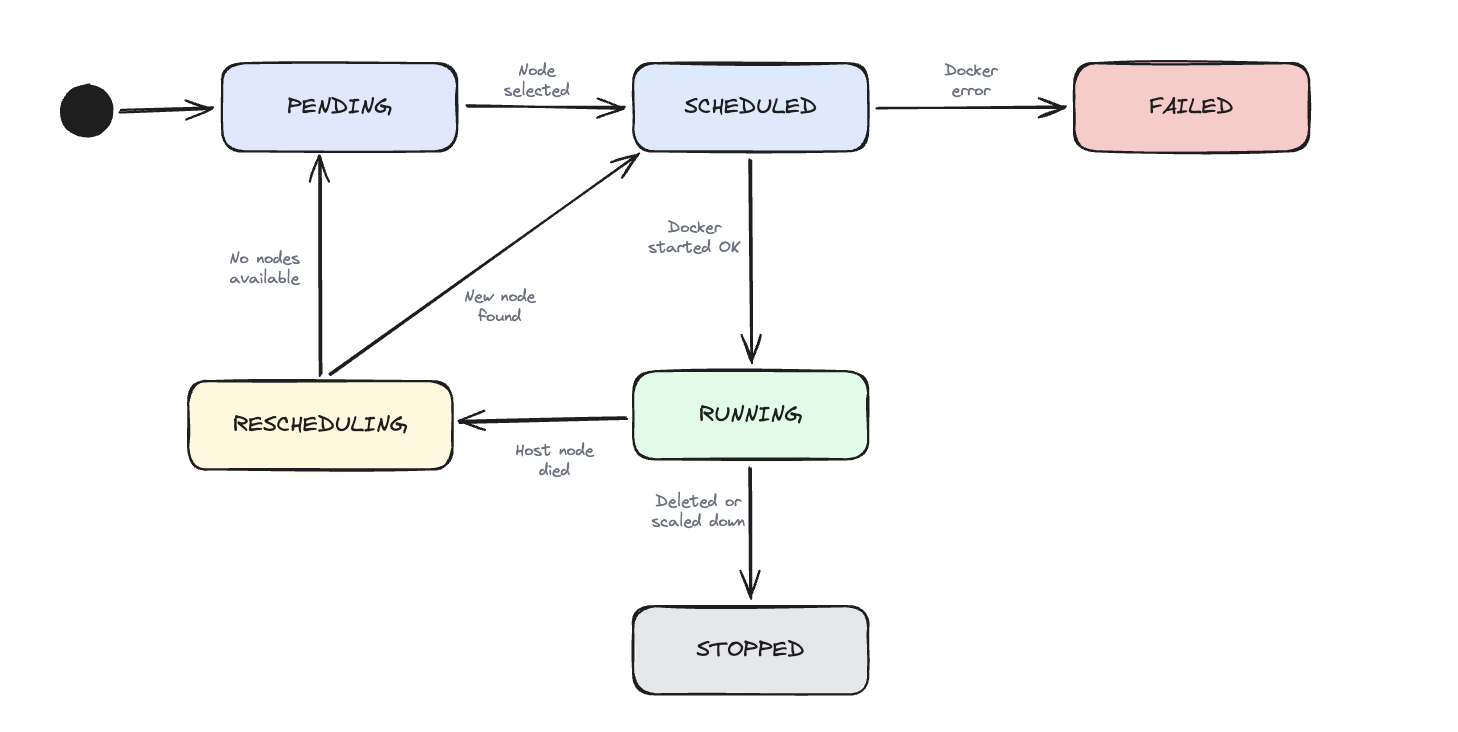
\includegraphics[width=\textwidth]{continut/capitol3/figuri/container_state_machine.png}
    \caption{Container -- State Machine}
    \label{fig:container_state_machine}
\end{figure}

A container goes through the following states:

\begin{itemize}
    \item \textbf{PENDING} -- the container needs to run, but no node has enough resources. It waits until resources become available.
    \item \textbf{SCHEDULED} -- a node was found and the container has been assigned. Docker startup is in progress.
    \item \textbf{RUNNING} -- Docker started the container successfully. This is the normal operating state.
    \item \textbf{FAILED} -- Docker returned an error (invalid image, port conflict, out of memory). The system will retry on another node.
    \item \textbf{RESCHEDULING} -- the host node died. A fresh container needs to be started on another node.
    \item \textbf{STOPPED} -- the container was stopped intentionally (service deleted or scaled down). This is a final state.
\end{itemize}

\section{Implementation}

The platform is structured as a single Go module with two binaries: \texttt{master} and \texttt{worker}. The following packages have been implemented:

\begin{itemize}
    \item \texttt{internal/domain} -- data models (Node, Service, Container, ResourcePool, User, AuditEntry, Heartbeat)
    \item \texttt{internal/cluster} -- in-memory cluster state with thread-safe CRUD operations, protected by \texttt{sync.RWMutex}
    \item \texttt{internal/heartbeat} -- UDP multicast sender (worker) and receiver (master) with auto-join on first heartbeat
    \item \texttt{internal/fault} -- fault tolerance: periodic health checks, SUSPECT/DEAD detection, KillContainers for split-brain prevention
    \item \texttt{internal/loadbalancer} -- LoadBalancer interface with LeastConnections and Weighted implementations
    \item \texttt{internal/scheduler} -- filters nodes by pool and resources, delegates to Load Balancer for node selection
    \item \texttt{internal/agent} -- TCP command server (StartContainer, KillContainers), system metrics monitor (CPU, RAM), and command client for master-to-worker communication
\end{itemize}
